%% =============================================================================
%% ОБЩИЕ ПРАВИЛА (для людей и для ИИ-агентов)
%% =============================================================================
%% 1. Это черновик ОДНОГО участника. Редактируй только этот файл.
%% 2. Не меняй чужие файлы в папке drafts/.
%% 3. Не трогай корневой main.tex, преамбулу, стили (.cls, .sty), .github/.
%% 4. Можно использовать существующие метки (
ef, \label, \cite), но не переименовывай их без согласования.
%% 5. Новые рисунки складывай в figures/ с уникальным именем: <имя>_<смысл>.png.
%% 6. Новые источники (BibTeX) пришли Давиду (david_final.tex) или в issues.
%% 7. Сохраняй статью в формате IEEEtran; не меняй шрифты/поля.
%% 8. После правки скинь файл координатору; сборка PDF делается в main.tex.
%% =============================================================================

%% УЧАСТНИК: Женя
%% РАЗДЕЛЫ: PLCnext and AXC F 2152 + Developed Neuro-PID controller
%% ЗАДАЧИ:
%%   - Сжать общее описание PLCnext/AXC F 2152 до 1 страницы.
%%   - Сделать акцент на интеграции PLCnext с OSTIS и нейро-ПИД.
%%   - Переписать раздел Neuro-PID (формулы оставить, текст — другой).
%%   - Обновить рисунки Neuro-adjuster-PID.png и pic_developed_NN*.png.
%%   - Добавить источники по нейро-ПИД 2024-2025.
%% =============================================================================

\section{PLCnext and AXC F 2152}

The neural network will be deployed on PLCnext controllers.

PLCnext Control is the hardware platform of PLCnext technology, providing an
open Linux environment with access to more data through Internet of Things
systems and greater flexibility. In addition to standards such as IEC 61131,
parallel programming and a combination of programming languages such as C/C++,
C\#, or MATLAB® Simulink® are also possible in real time with PLCnext Control.
There are three different categories of PLCnext control: flexible modular
controllers, high-performance remote field controllers, and iPC-based
controllers.

The advantages of the PLCnext platform, together with the chosen deployment
method, make it possible to effectively apply the developed neural network.

In this project, the PLCnext Technology Starterkit is used as the control device
(see Figure \ref{fig:ACXF2152}). This kit includes everything needed to work
with PLCnext technology for industrial automation. The kit contains the control
device — an \textbf{AXC F 2152} controller — AXL Smart Elements DI16/DO16/AI4
I/O modules, a slide potentiometer, an Ethernet cable, a starter kit manual, and
a link to a modeling file. The kit is designed to provide a simple, convenient,
and cost-effective way to start projects using PLCnext technology. With this
kit, users can test the operation, control, and high performance of PLCnext
technology on a compact station. The PLCnext Starterkit comes with detailed
documentation and a user manual that help developers get started quickly. It can
also provide access to online courses and materials for additional training and
deepening knowledge of PLCnext.

\begin{figure}[ht]
    \centering
    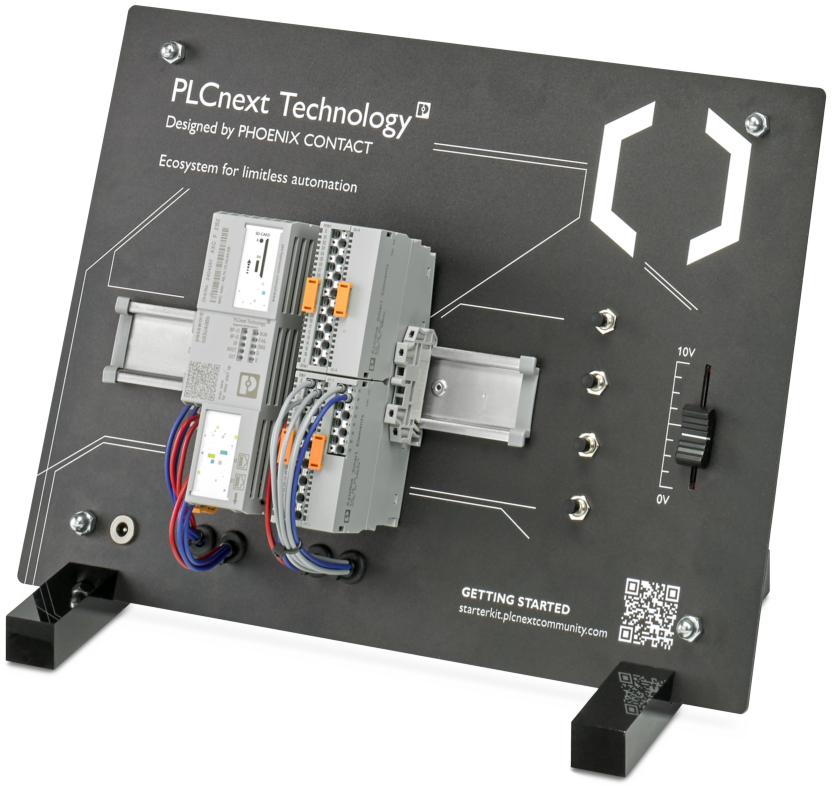
\includegraphics[width=0.45\textwidth]{figures/plcnext_x.png}
    \caption{PLCnext Technology Starterkit}
    \label{fig:ACXF2152}
\end{figure}

Let us now look in more detail at the “heart” of the platform — the AXC F 2152
controller. The controller has powerful computing capabilities, various I/O
interfaces, and support for multiple programming languages.

Detailed technical specifications of the \textbf{AXC F 2152}:

\begin{itemize}

    \item[-] Processor:
        \begin{itemize}
            \item[•] CPU: dual-core ARM Cortex-A9.
            \item[•] Processor frequency: 800 MHz.
            \item[•] Built-in memory: 1 GB RAM, 4 GB eMMC.
        \end{itemize}

    \item[-] Communication interfaces:
        \begin{itemize}
            \item[•] Ethernet: 2 x 10/100/1000 Mbps.
            \item[•] USB: 2 x USB 2.0 Host.
            \item[•] RS232: 1 x port with RTS/CTS support.
        \end{itemize}

    \item[-] Inputs/outputs:
        \begin{itemize}
            \item[•] Digital inputs: 16 x 24 V DC, with counter support.
            \item[•] Digital outputs: 16 x 24 V DC, maximum current 500 mA per
            output.
            \item[•] Analog inputs: 2 x 0-10 V, 12-bit resolution.
            \item[•] Analog outputs: 2 x 0-10 V, 12-bit resolution.
        \end{itemize}

    \item[-] Expansion:
        \begin{itemize}
            \item[•] Expansion slots: 2 x PLCnext expansion module slots.
            \item[•] Support for expansion modules: I/O modules, communication
            interface modules, and additional functional modules.
        \end{itemize}

    \item[-] Power:
        \begin{itemize}
            \item[•] Supply voltage: 24 V DC.
            \item[•] Power consumption: up to 18 W.
        \end{itemize}

    \item[-] Operating system:
        \begin{itemize}
            \item[•] PLCnext Runtime: based on Linux.
        \end{itemize}

    \item[-] Software:
        \begin{itemize}
            \item[•] Supported programming languages: IEC 61131-3 (ST, LD, FBD,
            SFC), C++, C\#, Python.
            \item[•] Built-in software: PLCnext Engineer, PLCnext Runtime.
        \end{itemize}

    \item[-] Operating conditions:
        \begin{itemize}
            \item[•] Operating temperature: 0°C to 55°C.
            \item[•] Humidity: 5\% to 95\%, non-condensing.
        \end{itemize}

\end{itemize}

The main components of the \textbf{AXC F 2152} (modules, interfaces) are shown
in Figure \ref{fig:PLCComplect}.

\begin{figure}[ht]
    \centering
    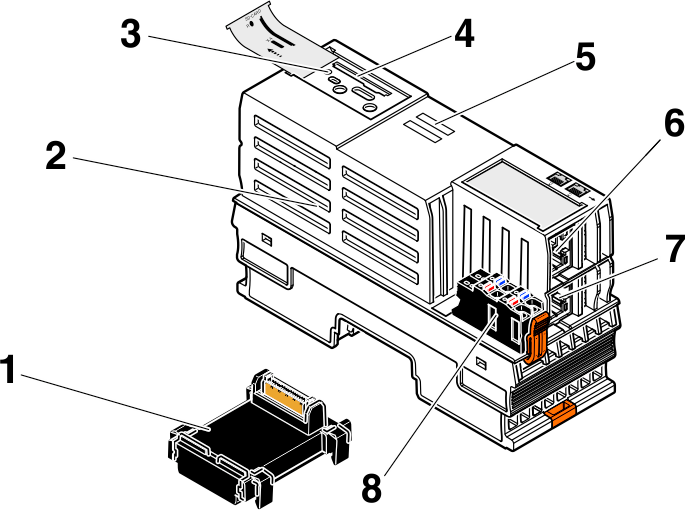
\includegraphics[width=0.45\textwidth]{figures/plcnext_complect.png}
    \caption{Components of the \textbf{AXC F 2152}}
    \label{fig:PLCComplect}
\end{figure}

The controller includes:

\begin{enumerate}
    \item Basic bus module.
    \item Electronics module.
    \item Reset button.
    \item SD cardholder.
    \item Diagnostic and status indicators.
    \item Ethernet interface (1).
    \item Ethernet interface (2).
    \item Power connector.
\end{enumerate}

To connect various peripherals to the \textbf{AXC F 2152}, the following steps
must be taken:

\begin{enumerate}
    \item Use the base bus module to connect the controller to the Axioline F
    local bus, which can support up to 63 I/O devices.
    \item Use the Ethernet interface(s) to connect the controller.
    \item Configure the network and controller settings.
    \item Create a new project, add the controller and peripheral devices to the
    hardware configuration.
    \item Download the project to the controller and start it.
\end{enumerate}

Various Axioline F I/O devices can be connected to the \textbf{AXC F 2152}, such
as:

\begin{itemize}
    \item[-] Digital I/O modules (for example, DI8/1 DO8/1 2701916) for handling
    discrete signals.
    \item[-] Analog I/O modules (for example, AI2 AO2 2702072) for handling
    analog signals.
    \item[-] Special-purpose modules (for example, AXF BK PN 2701815) for
    connection to other buses.
\end{itemize}

The AXC F 2152 PLCnext Control controller has high performance, a variety of
communication interfaces, scalability, and support for multiple programming
languages. It is well suited for process automation, offering flexibility,
reliability, and ease of development.

\subsection{Development with PLCnext}

The neural network was developed on Windows using Visual Studio 2022. To deploy
on PLCnext controllers, these projects must be built for the target platform.

Visual Studio is a powerful and popular integrated development environment (IDE)
from Microsoft. The following advantages led to choosing it as the most suitable
tool for the project:

\begin{itemize}

    \item[-] Rich functionality. Visual Studio Community provides a wide range
    of tools and capabilities for developing and debugging software. It supports
    various programming languages, including C++, C\#, Visual Basic, Python, and
    others that can be used with the PLCnext SDK. Visual Studio also includes
    tools for debugging, profiling, version control, and automation.

    \item[-] Integration with other tools. Visual Studio Community integrates
    with various development services and tools, which simplifies working with
    them. Visual Studio includes the PLCnext Technology Development Tools
    extension, which adds project templates and elements, as well as a debugging
    module for PLCnext Technology. VS also supports CMake, which is the build
    system for this project.

    \item[-] Availability. Visual Studio Community is free for non-commercial
    use, including academic and personal projects. This helps reduce licensing
    costs for the development environment.

\end{itemize}

PLC Toolchain will be used for programming the controller. It is a set of tools
for programming logic controllers in high-level languages such as C++ and C\#.
It enables the use of these languages to create complex, efficient control
algorithms and to integrate with other systems and technologies.

PLC Toolchain is based on the \textbf{Beremiz} development environment, which
complies with the IEC 61131-3 standard. This standard defines five programming
languages for PLCs: Instruction List, Symbolic Flowchart, Ladder Diagram,
Function Block Diagram, and Structured Text. PLC Toolchain allows these
languages to be used in combination with C++ and C\#, and also supports code
portability across different platforms and hardware.

PLC Toolchain includes tools for creating Human-Machine Interfaces (HMIs) and
for connecting PLC programs to existing databases and fieldbuses.

The PLCnext SDK is also required to work with the PLCnext platform and the AXC F
2152 controller. It is a set of tools for developing applications for PLCnext
Technology controllers in different programming languages. The PLCnext SDK
includes compilers, debuggers, libraries, and other resources needed to create
native applications for the target device. PLCnext SDK is installed and managed
via the command line interface (CLI) called PLCnext CLI, or \textbf{plcncli}.

\subsection{Installation of PLCnext}

After the neural network has been built, the resulting executable needs to be
transferred to the existing controller.

For this task, several options can be used:

\begin{itemize}
    \item[-] WinSCP combined with PuTTY 64-bit.
    \item[-] Specialized PLCnext Engineer software tools.
\end{itemize}

These tools each have their own advantages and disadvantages. Let us describe
them.

The main advantage of PLCnext Engineer is that it is specifically tailored to
the PLCnext technology. PLCnext Engineer is an engineering suite for developing
automated solutions based on controllers. It includes all the engineering
disciplines necessary for the full development and commissioning of an
automation project. These engineering tasks include:

\begin{enumerate}
    \item Network configuration.
    \item Development of application code.
    \item HMI (Human-Machine Interface).
    \item OPC UA server.
\end{enumerate}

These functions make PLCnext Engineer a highly suitable tool for deploying the
developed program to the controller.

However, PLCnext Engineer is not the only alternative. To make an informed
choice, it is worth considering other tools such as PuTTY combined with WinSCP.

PuTTY is an SSH and telnet client originally developed by Simon Tatham for the
Windows platform. PuTTY is open-source software, available with source code and
maintained by a group of volunteers.

WinSCP is a free open-source SFTP client, FTP client, WebDAV client, S3 client,
SCP client, and file manager for Windows. Its primary function is file transfer
between local and remote computers. In addition, WinSCP provides scripting and
basic file manager features.

WinSCP provides:

\begin{itemize}
    \item[-] A graphical user interface.
    \item[-] Support for multiple languages.
    \item[-] Integration with Windows (drag-and-drop, URLs, quick access icons,
    navigation history).
    \item[-] Common file operations for both local and remote files.
    \item[-] Support for SFTP and SCP over SSH, as well as FTP, WebDAV, and S3.
    \item[-] A scriptable command-line interface and .NET assembly for advanced
    programming tasks.
    \item[-] Directory synchronization using several semi-automatic modes.
    \item[-] A built-in text editor.
    \item[-] Shared site storage with PuTTY.
    \item[-] Authentication support using password, keyboard-interactive, public
    key, and Kerberos (GSS).
    \item[-] Integration with Pageant (PuTTY authentication agent) for full SSH
    public key authentication support.
    \item[-] A file explorer and interface manager.
    \item[-] Optional protection of saved site information with a master
    password.
    \item[-] Optional portable mode using a configuration file instead of
    registry entries, suitable for removable media.
\end{itemize}

This choice was made because these programs are simple, highly functional, and
together can cover all necessary requirements for transferring the compiled
neural network executable to the controller.

\subsection{Porting to PLCnext}

The following components will be used to build the program for the controller:

\begin{enumerate}
    \item CMake (build system).
    \item \textbf{plcncli} (command line for PLCnext controllers).
    \item SDK for the selected controller.
\end{enumerate}

To successfully build the program for the selected controller, CMake must be
installed on the computer. This tool provides the ability to perform
cross-platform builds for different targets.

After CMake is installed, the \textbf{plcncli} command line must be installed to
download the selected SDKs and build programs for the target controller. It
provides the necessary build tools.

After \textbf{plcncli} has been installed, you need to download and install the
SDK from the official site using the \textbf{plcncli} command:

\begin{lstlisting}[basicstyle=\ttfamily\small,breaklines=true,breakatwhitespace=true]
plcncli.exe install sdk -d [installation path] -p [path to archive file]
\end{lstlisting}

After the SDK is installed, you need to open Visual Studio and configure the
CMake project for the controller.

\section{Developed Neuro-PID controller}

The overall structure of the self-tuning Neuro-PID controller is shown in Fig.
\ref{fig:neuro_PID_controller}, where the neural network (NN) outputs are
proportional ($K$), integral ($T_I$), and differential ($T_d$) components
\cite{ivaniuk2013neuro}.

\begin{figure*}[ht]
  \centering
  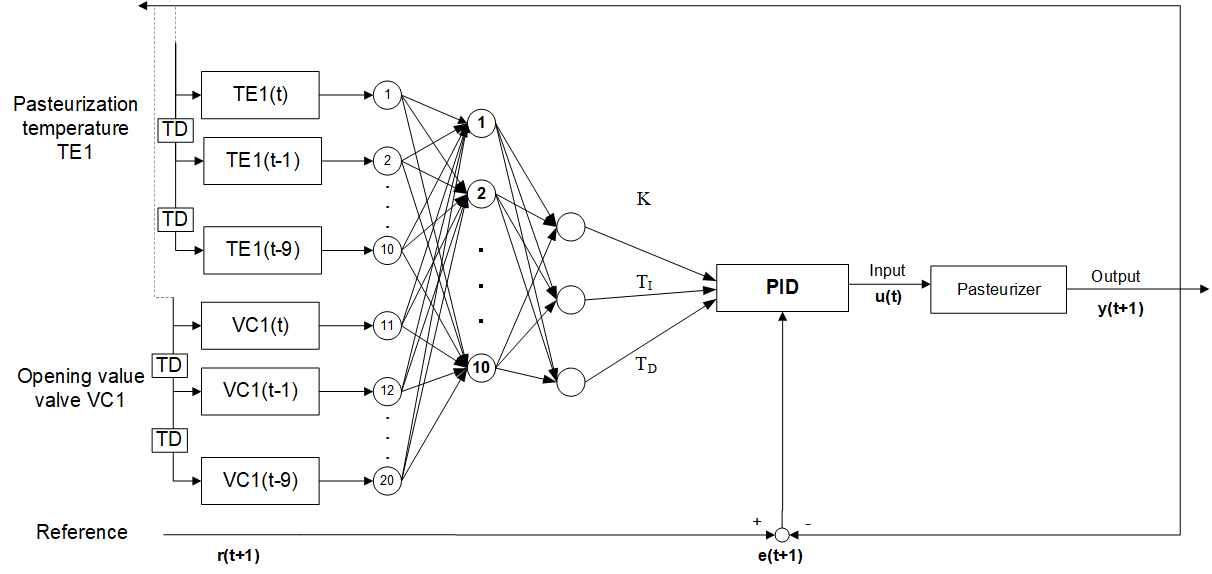
\includegraphics[width=\textwidth]{figures/pic_developed_NN_full.png}
  \caption{The developed Neuro-PID controller (TD means delay operator)}
  \label{fig:neuro_PID_controller}
\end{figure*}

To control the Pasteurizer \cite{ivaniuk2013neuro}, a PID controller is
configured with a multilayer perceptron (MLP, neuro-PID adjuster) with the
following structure: 20 input, 10 hidden and 3 output neural elements; the
activation function for the hidden and output layers is sigmoid.

The discrete-time \textbf{PID controller} can be described by equation
\ref{PID_algorithm} \cite{ivaniuk2013neuro}, where $P$, $T_I$ and $T_D$ are
proportional factors, integral and differential constituents respectively, $u_n$
determines the input of a control object at a time of $t = n T_0$ and $e_n$ — an
error between the desired output value of $r_n$ and the real output of $e_n =
r_n - y_n$. $T_0$ defines a unit time interval.

\begin{equation}\label{PID_algorithm}
  \begin{aligned}
    u_k  & = u_{k - 1} + \Delta u_k,                                         \\
    \Delta u_k & = q_0 e_k + q_1 e_{k - 1} + q_2 e_{k - 2},                  \\
    q_0  & = \mathbf{K}\left(1 + \frac{T_D}{T_0}\right),                     \\
    q_1  & = -\mathbf{K}\left(1 + 2\frac{T_D}{T_0} - \frac{T_0}{T_I}\right), \\
    q_2  & = \mathbf{K}\frac{T_D}{T_0}.
  \end{aligned}
\end{equation}

Algorithm for operation of \textbf{neuro-PID adjuster} \cite{ivaniuk2013neuro}:

\begin{equation}\label{PID_nn}
  \begin{aligned}
    y_j       & = F(\sum_{i}{\omega_{i j}y_i - T_j}),                         \\
    \gamma_j  & = y_j - t_j,                                                  \\
    \gamma_i  & = \sum_{i}{\gamma_iF^\prime(S_i)\omega_{j i}},                \\
    \omega_{i j}(t + 1) & = \omega_{i j}(t) - \alpha\gamma_jF^\prime(S_j)y_i, \\
    T_j(t + 1)& = T_j(t) + \alpha\gamma_jF^\prime(S_j),                       \\
    E         & = \frac{1}{2}\sum_{k = 1}^{L}{\sum_{j}{({y_j}^k} - {t_j}^k)^2}.
  \end{aligned}
\end{equation}

To use the back propagation algorithm, we must select the $E$ function, which
must be minimized. It will be the management error $e_n$ at the time $t = n
T_0$, so $E_n = \frac{1}{2}e_n^2$. To accumulate errors, we store the data we
have previously obtained — $E_{n-p},... E_{n-2},E_{n-1},E_n$, where $p$
determines the number of previously saved images used for network learning
(\ref{PID_nn}).

